\section{Empirical validation}\label{sec:experiments}
In this section, we provide empirical validation of our end-to-end \textsc{QuaRK} model. The goal is to empirically support our two key learning-theoretic guarantees outlined in our theoretical analysis. First, we study the capacity of our model to effectively learn the selected tasks by showing that the training mean-squared error decreases smoothly and reaches zero beyond a finite threshold as we sweep the readout complexity, thereby corroborating the existence of an interpolation regime for our method. Second, we study our model's generalization capacity. Once trained in this effective-learning regime, we evaluate the out-of-sample performance of the model and demonstrate that the test error decreases as we increase the number of training windows, which aligns with the scaling suggested by our generalization bound. In order to keep the empirical study compact and highly interpretable, we focus on a synthetic $\beta$-mixing vector autoregressive moving average (VARMA) family and representative DGP functionals with varying complexity. The experiments were conducted using Qiskit~\cite{javadi2024quantum}, and the quantum circuits were simulated on a simulator using a machine with two Nvidia A100 GPUs. Code available here \href{https://github.com/abdo-aary/quark}{https://github.com/abdo-aary/quark}.

\subsection{Empirical set up}
For all the experiments, we generate a multivariate input process $\rmX = (X_t)_{t \leq 0} \in \gIZ$, with $\gI := (-1,1)^d$ and $d=3$, from a $\VARMA(p,q)$ recursion with $p = q = 3$ (to allow multistep dependencies), given as
\begin{equation}
    Z_t=\sum_{i=1}^p\Phi_i Z_{t-i}+\Theta_0\epsilon_t+\sum_{j=1}^q \Theta_j \epsilon_{t-j}, \qquad X_t := \tanh(Z_t),
\end{equation}
where $(\epsilon_t)$ are i.i.d.\ centered innovations, and the AR part satisfies the usual stability conditions to allow the $\beta$-mixing property (see Appendix~\ref{subsec:VARMA} for details). From a trajectory, we form supervised examples by sliding windows of length $w$, $\rmX_t := (X_{t-w+1}, \ldots, X_t)$, along with a scalar label $Y_t \in \sR$, with $w = 25$ and a stride $s = 100$ (i.e.\ gap $g = 75$). Labels are generated by fixed ground-truth fading-memory functionals $H^\star: \gIZ \to \sR$, whose window-truncated versions $H^\star_w$ are used so that $Y_t = H^\star_w (\rmX_t)$.

We consider three functionals (tasks) chosen with varying difficulty. The first and easiest task is a one-step forecasting functional $H^\star_{\rm fore}(\boldsymbol{X}_t) := u^\top X_{t+1}$, with $u \in \sR^d$ defining a fixed projection, which depends linearly only on the immediate future. The second, more difficult task is an exponentially fading linear functional, which involves decaying memory over many lags in a linear fashion,
\begin{equation}\label{eq:exponential-fading-linear}
    H^\star_{\rm exp}(\boldsymbol{X}_t)
    := \sum_{k\geq0}\alpha^k\, u^\top X_{t-k},
    \quad
    Y_t := H^\star_{{\rm exp},w}(\boldsymbol{X}_t)
    := \sum_{k=0}^{w-1}\alpha^k\, u^\top X_{t-k},
\end{equation}
with $\alpha \in (0,1)$, thereby requiring the learning model to aggregate information across the whole window while capturing the decaying importance. The final and most difficult task is related to a Volterra-type functional of order two, which adds quadratic cross-lag interactions to the fading memory term in~\cref{eq:exponential-fading-linear},
\begin{equation}\label{eq:volterra-functional}
    H^\star_{\rm vol}(\boldsymbol{X}_t)
    = \sum_{k\geq0}\alpha^k\, u^\top X_{t-k}
    + \frac{1}{2}\sum_{k\geq0}\sum_{\ell\geq0}\alpha^{k+\ell}\,
    (v^\top X_{t-k})(v^\top X_{t-\ell}),
\end{equation}
with $v  \in \sR^d$ defining a fixed projection, and where $H^\star_{{\rm vol}, w}$ is obtained by truncating $k,\ell \in \{0, \ldots, w-1\}$.

\subsection{Learning theory validation}
We used $n = 5$ qubits per sub-reservoir to align the empirical study with the projection-dimension guideline proposed in Section~\ref{subsubsec:projection}. This matches the prescribed scaling $n \approx \log(w N)$ for the JL projection dimension, with $w = 25$ and a maximum number of training windows of $N=8000$. This choice is made for the two experiments below in order to fix the quantum featurizer complexity while probing the emergence of an interpolation regime by sweeping the readout norm budget and testing the generalization bound's sample-size behavior by varying the number of training windows up to $N=8000$.

Embeddings $H^T(\rmX)$ are probed following the classical-shadows measurement strategy on the $2$-local Pauli observable set. We perform $1000$ measurement shots (classical snapshots) per circuit to construct the feature vector $m \circ H^T(\rmX)$. 
A number of $R=3$ independent sub-reservoirs are used to obtain a rich representational capacity. Throughout all the experiments, the architecture of each sub-reservoir is fixed to be the ring architecture and unitary pattern illustrated in Figure~\ref{fig:unitary-evolution}.


\subsubsection{Effective learning validation}
\begin{figure}
    \centering
    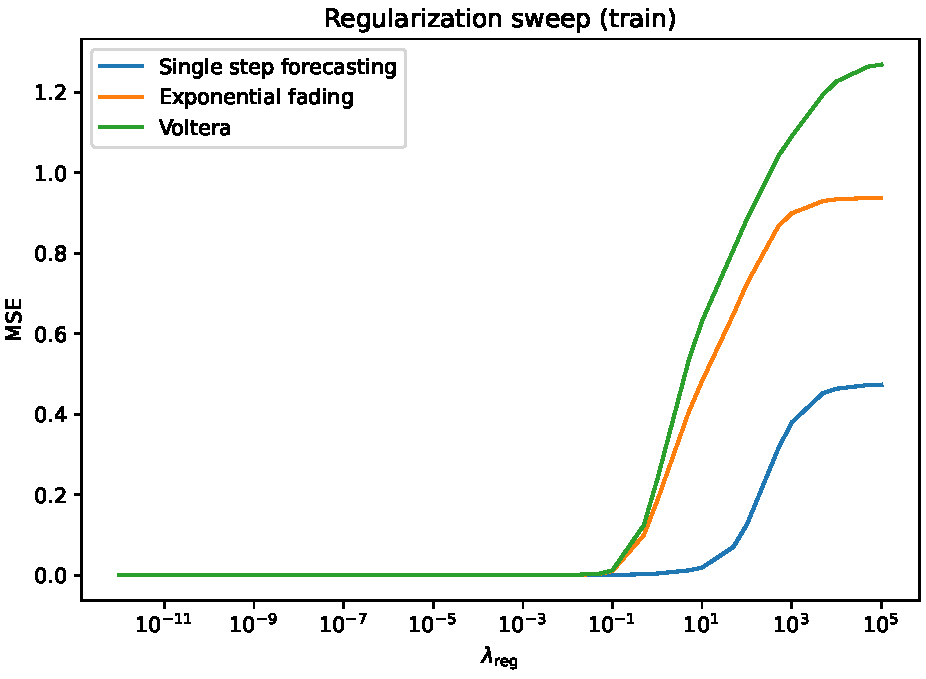
\includegraphics[width=0.8\linewidth]{figs/train_regularization.pdf}
    \caption{\small Training MSE versus the readout regularization $\lambda_{\rm reg}$ for the three functionals, featuring a sharp transition into the interpolation regime around $\lambda_{\rm reg} \approx 10^{-1}$, where the curves reach numerical zero.}
    \Description{Line plot of training mean-squared error versus the readout regularization strength on a logarithmic horizontal axis. Three curves are shown: single-step forecasting, exponential fading, and Volterra. For very small regularization, all curves stay near zero error (interpolation regime). Around a regularization value near 0.1, the error increases sharply. The Volterra curve rises the most, exponential fading rises next, and single-step forecasting remains the lowest among the three.}
    \label{fig:regularization-sweep}
\end{figure}

The first experiment validates the effective-learning prediction of our theoretical analysis in Section~\ref{subsec:effective-learning} by isolating a single control parameter: the readout complexity. Concretely, we fix all experimental choices, including the quantum featurizer, and we perform a sweep over the regularization parameter $\lambda_{\rm reg}$ (equivalently, a sweep over the RKHS norm budget $\Lambda$). Figure~\ref{fig:regularization-sweep} reports the training MSE for each of the three tasks as a function of the regularization parameter. The key observation in this figure is the existence of a clear transition point into an interpolation regime, where, as we relax the constraint, the training error decreases and eventually reaches numerical zero in a smooth fashion. This is precisely what is predicted by Theorem~\ref{thm:effective-learning}: beyond a finite threshold, the readout hypothesis class becomes rich enough to push the empirical risk to zero. Furthermore, Figure~\ref{fig:train-fit} illustrates the fit on a subset of training windows in the interpolation regime, where we visualize predictions against ground-truth labels. This shows perfect fitting of the training dataset and highlights that the low training loss reported in Figure~\ref{fig:regularization-sweep} is not merely an artifact of averaging.


\begin{figure}
    \centering
    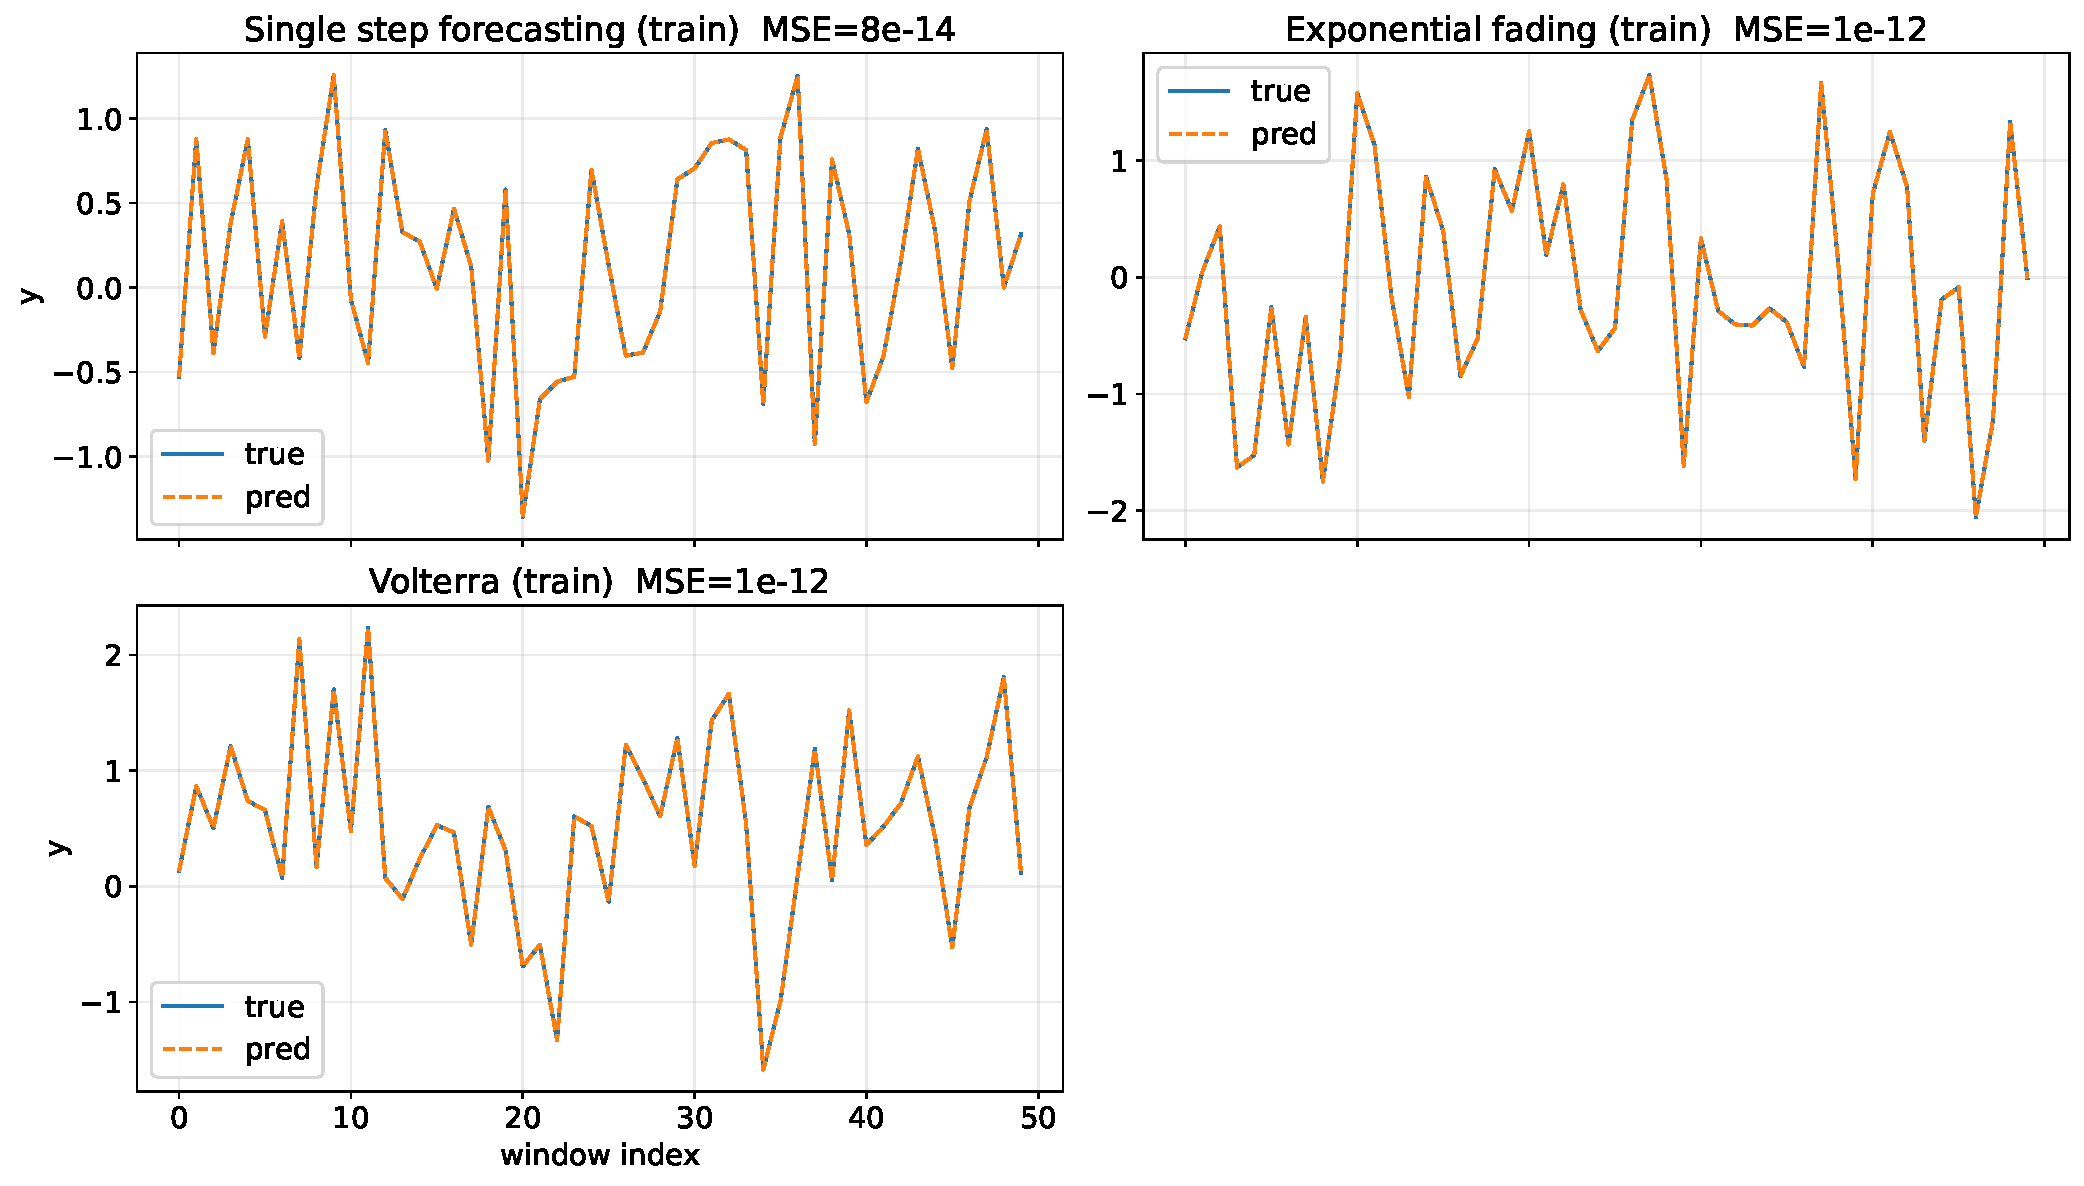
\includegraphics[width=\linewidth, height=6cm]{figs/true_vs_pred_grid_test.pdf}
    \caption{\small Predicted vs true labels on a subset of training windows for the three functionals from the interpolation regime. Numerical errors reach values of ${\rm MSE} \in [10^{-14}, 10^{-12}]$ confirming perfect task learning.}
    \Description{Three time-series panels comparing ground-truth outputs (“true”, solid line) to model predictions (“pred”, dashed line) over window index (about 0 to 50) for single-step forecasting, exponential fading, and Volterra tasks. In all panels, the predicted curve is visually indistinguishable from the true curve, indicating near-perfect fit on the training windows, consistent with the extremely small reported training MSE values in the panel titles.}
    \label{fig:train-fit}
\end{figure}

\subsubsection{Generalization guarantee validation}\label{subsubsec:generalization-validation}
In this second experiment, we experimentally validate the claim made in Theorem~\ref{thm:generalization}. We first fix all modeling choices to a single configuration: same kernel, same quantum featurizer, and a single fixed readout regularization $\lambda_{\rm reg}$ chosen to be sufficiently relaxed. Then, we sweep the number of training windows $N$ from $100$ to $8 \cdot 10^3$, where for each value of $N$, we train the same kernel readout on the corresponding training subset and record the out-of-sample MSE on a fixed held-out test set. Figure~\ref{fig:varying-datasizes} illustrates that the test error decreases as $N$ increases across the three tasks, which aligns with the scaling predicted by the bound in~\cref{eq:bound-generalization}. Importantly, the decay of the three curves follows the same $\tfrac{1}{\sqrt{N}}$ shape (up to additional constants), thereby validating the prediction made in Section~\ref{subsubsec:generalization}. Furthermore, the ranking of the obtained test MSE values reflects the relative hardness of the functionals: the single-step forecasting functional yields the lowest values, followed by the exponential-fading and Volterra functionals.

\begin{figure}
    \centering
    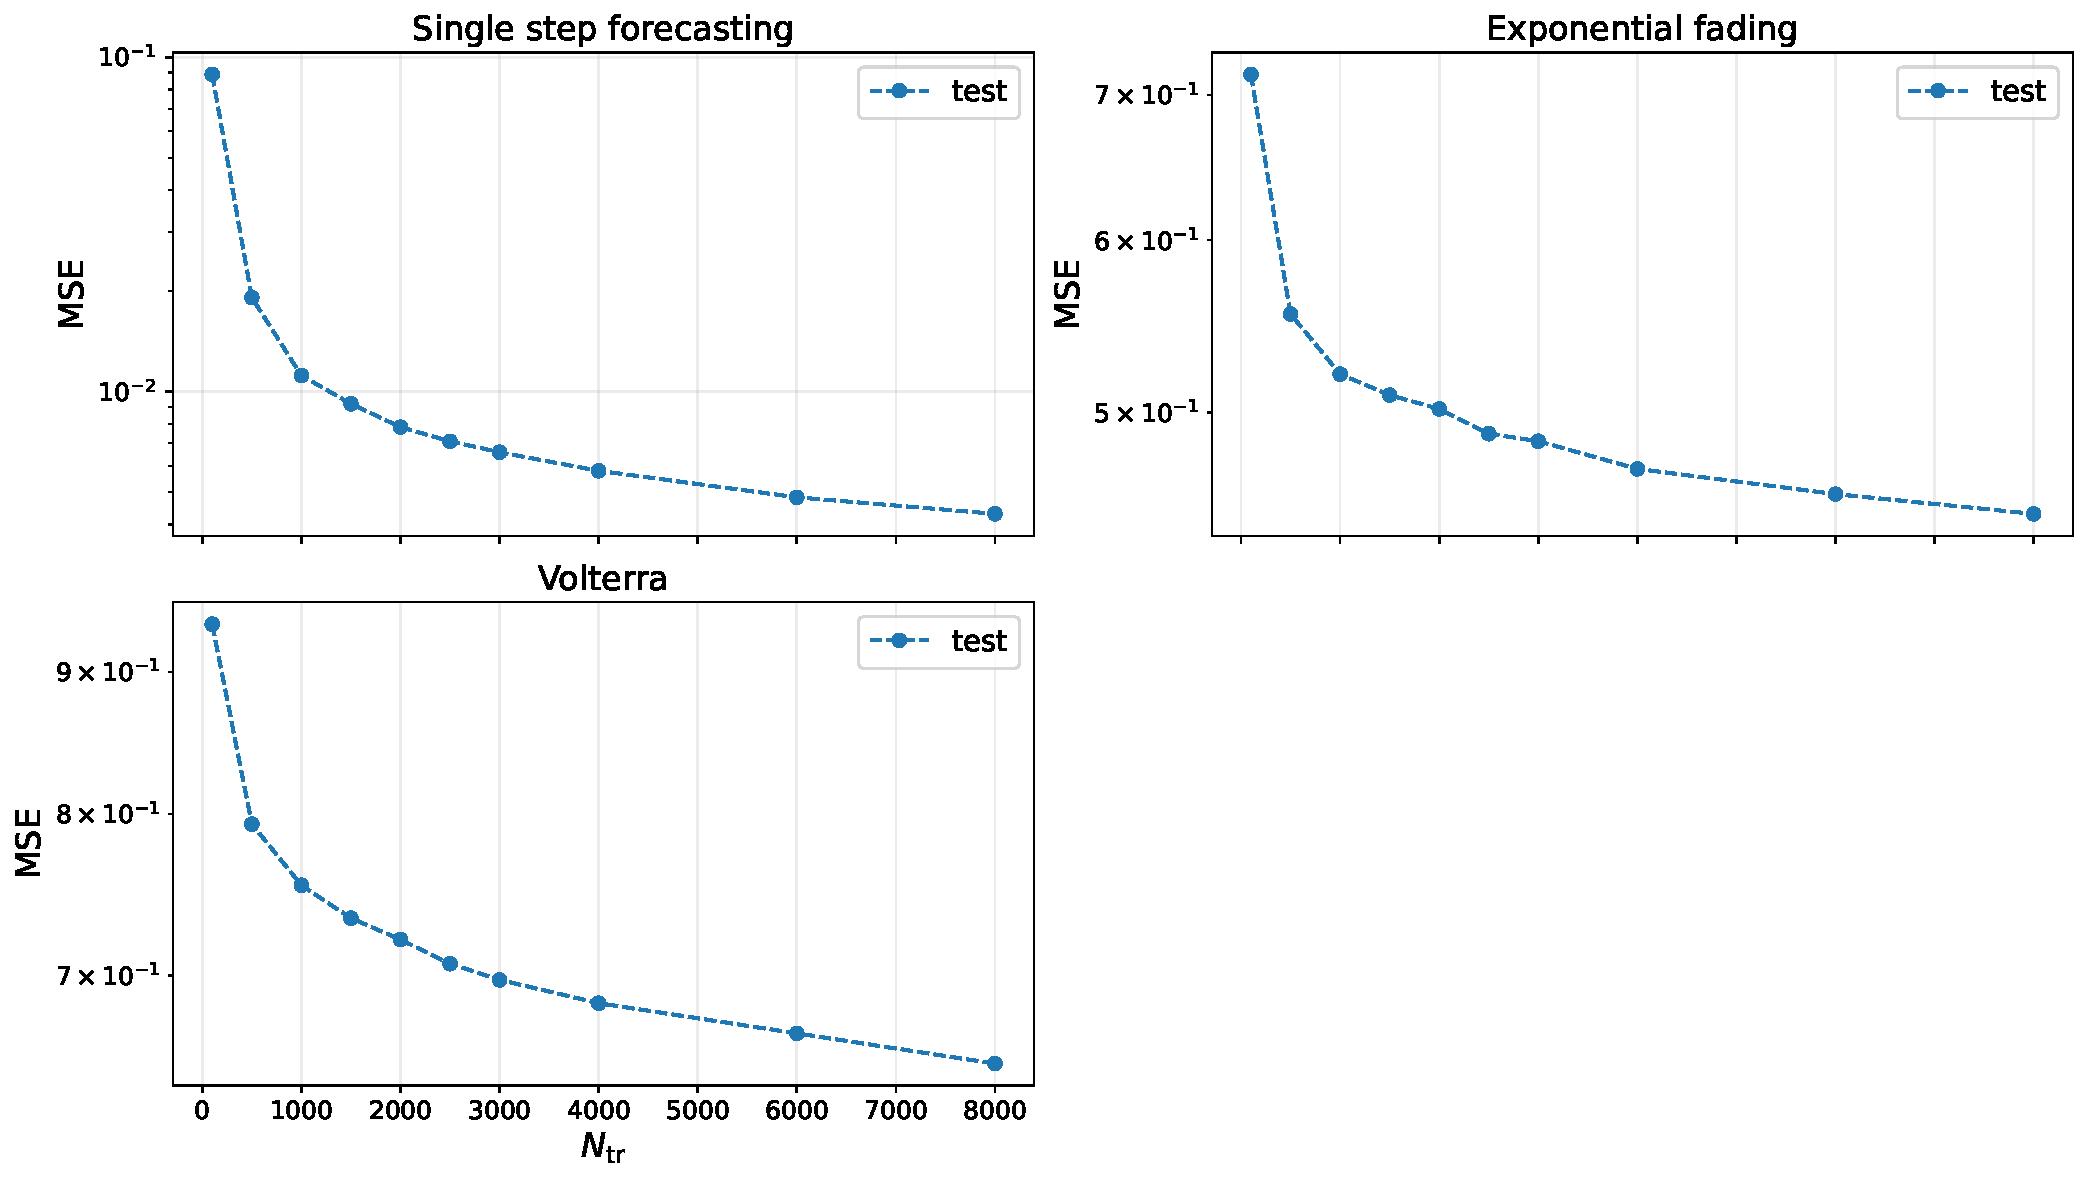
\includegraphics[width=\linewidth, height=6cm]{figs/test_mse_vs_varying_dataset_sizes.pdf}
    \caption{\small Test MSE vs training-set size $N$ reported for the three tasks, obtained by sweeping $N$ while keeping the other experimental choices, and reported for a same held-out test split.}
    \Description{Three panels showing test MSE as a function of training-set size N for single-step forecasting, exponential fading, and Volterra. In each panel, a dashed line with markers decreases as N increases, indicating improved generalization with more training data. The single-step task shows the steepest drop, while exponential fading and Volterra decrease more gradually but consistently over the full range of N.}
    
    \label{fig:varying-datasizes}
\end{figure}

% \subsection{Comparison against classical benchmarks}

% Context: training-size sweep (fixed test set) + learning-curve visualization
%
% We ran a classical learning-curve experiment on a *fixed* dataset/model pair already loaded in `exp`
% (i.e., `exp.dataset` and a trained/loaded `exp.model` with cached features $\Phi_{\text{full}}$ so that
% no quantum circuits are re-executed).
%
% 1) Training-size sweep (nested training sets, fixed test set)
% -----------------------------------------------------------
% We called:
% \[
% \texttt{res} \leftarrow \texttt{sweep\_training\_sizes\_fixed\_test(exp, sizes, lambda\_regs=None, progress=True)}.
% \]
% Parameters:
% \begin{itemize}
%   \item \texttt{exp}: an \texttt{Experiment} instance with (i) a dataset of windowed VARMA samples and
%         associated labels for multiple tasks/functionals, and (ii) a KRR-style model already providing
%         cached feature vectors $\Phi_{\text{full}}$ for all windows (to avoid re-running the featurizer).
%   \item \texttt{sizes} $= [100, 500, 1000, 1500, 2000, 2500, 3000, 4000, 6000, 8000]$:
%         the list of training-set cardinalities $N_{\mathrm{tr}}$ to evaluate.
%         The procedure enforces nested subsets
%         $\mathcal{D}_{100}\subset \mathcal{D}_{500}\subset \cdots \subset \mathcal{D}_{8000}$
%         by taking prefixes of the ordered training indices.
%   \item \texttt{lambda\_regs=None}:
%         do \emph{not} re-select regularization by validation; instead, reuse the per-task best
%         regularization values $\lambda_\ell$ previously obtained from the regularization sweep stored
%         in the experiment artifacts. If the sweep is missing, the function raises an error.
%         The same fixed $\lambda_\ell$ is used for all $N_{\mathrm{tr}}$ values.
%   \item \texttt{progress=True}: show \texttt{tqdm} progress bars over tasks and training sizes.
% \end{itemize}
% Output:
% \texttt{res} is a dictionary keyed by $N_{\mathrm{tr}}$; each entry stores, per task/functionals,
% the fitted dual coefficients $\alpha_\ell$, predictions on train/test splits, and the resulting
% train/test MSE curves (notably \texttt{mse\_test} used below).
%
% 2) Visualization: test MSE vs training size, per task
% -----------------------------------------------------
% We then plotted learning curves using:
% \[
% \texttt{fig} \leftarrow \texttt{plot\_mse\_vs\_train\_size\_grid(res, exp=exp, split="test", ...)}.
% \]
% Parameters:
% \begin{itemize}
%   \item \texttt{res}: output of the training-size sweep above.
%   \item \texttt{exp=exp}: used to retrieve readable task/functionals names from the experiment.
%   \item \texttt{split="test"}: plot \emph{only} the test-set MSE, i.e., $\mathrm{MSE}_{\text{test}}(N_{\mathrm{tr}})$.
%   \item \texttt{panel\_titles} $=[\text{``Single step forecasting''},\ \text{``Exponential fading''},\ \text{``Volterra''}]$:
%         custom subplot titles, one per functional/task.
%   \item \texttt{y\_scale="log"}: logarithmic y-axis for MSE values.
%   \item \texttt{figsize=(14, 8)}: overall figure size.
%   \item Font controls:
%         \texttt{title\_fontsize=16}, \texttt{label\_fontsize=16}, \texttt{tick\_fontsize=12},
%         \texttt{legend\_fontsize=14}.
% \end{itemize}
% The resulting figure contains one panel per task showing the decay of test MSE as $N_{\mathrm{tr}}$
% increases from 100 up to 8000. (See the exported plot.) :contentReference[oaicite:0]{index=0}


% \subsection{Benchmarking against classical ESN}
